\subsubsection{Estimaci\'on de la Tasa de Descuento}

Cuanto mayor sea el riesgo sistem\'atico de una acci\'on, m\'as elevado ser\'a el rendimiento que los inversionistas esperar\'an de los t\'itulos accionarios. Con la finalidad de estimar una tasa de descuento apropiada en pesos, en t\'erminos nominales y despu\'es de impuestos, se utilizaron los siguientes insumos para determinar el valor del WACC:

\subsubsection{Costo de Capital accionario}

\textcolor{principal}{Tasa libre de riesgo (Rf).} Se basa en el rendimiento de los bonos gubernamentales, en este caso, se tom\'o en rendimiento del T-Bond americano, con el siguiente resultado:

\begin{figure}[H]
\centering
La tasa libre de riesgo obtenida es de \textbf{4.9479\%} \includegraphics[width=9cm]{imagenes/rf}
\end{figure}

\textcolor{principal}{Beta ($\beta$)}. Con la finalidad de determinar el factor beta apropiado para el negocio, se consider\'o las betas re-apalancadas del negocio.\\

\begin{figure}[H]
\centering
\includegraphics[width=17cm]{imagenes/beta_1}\\
\end{figure}
\begin{figure}[H]
\centering
\includegraphics[width=17cm]{imagenes/beta_2}
\end{figure}
\espacio{3cm}
\begin{figure}[H]
\centering
\includegraphics[width=17cm]{imagenes/beta_3}\\
\includegraphics[width=10cm]{imagenes/beta_4}
\end{figure}

La beta reapalancada y ponderada que corresponde a la empresa, es de \textcolor{principal}{\textbf{2.31x.}}

\espacio{1cm}



\textcolor{principal}{Prima de riesgo del mercado de capitales}. Se obtuvo del promedio hist\'orico de la diferencia de rendimientos o ``spread'' entre el mercado accionario mexicano mediante el indicador conocido como el ERP (enterprise risk premium).\\

\begin{figure}[H]
\centering
La prima de riesgo de mercado (ERP) es de \textbf{\textcolor{principal}{4.84\%}} 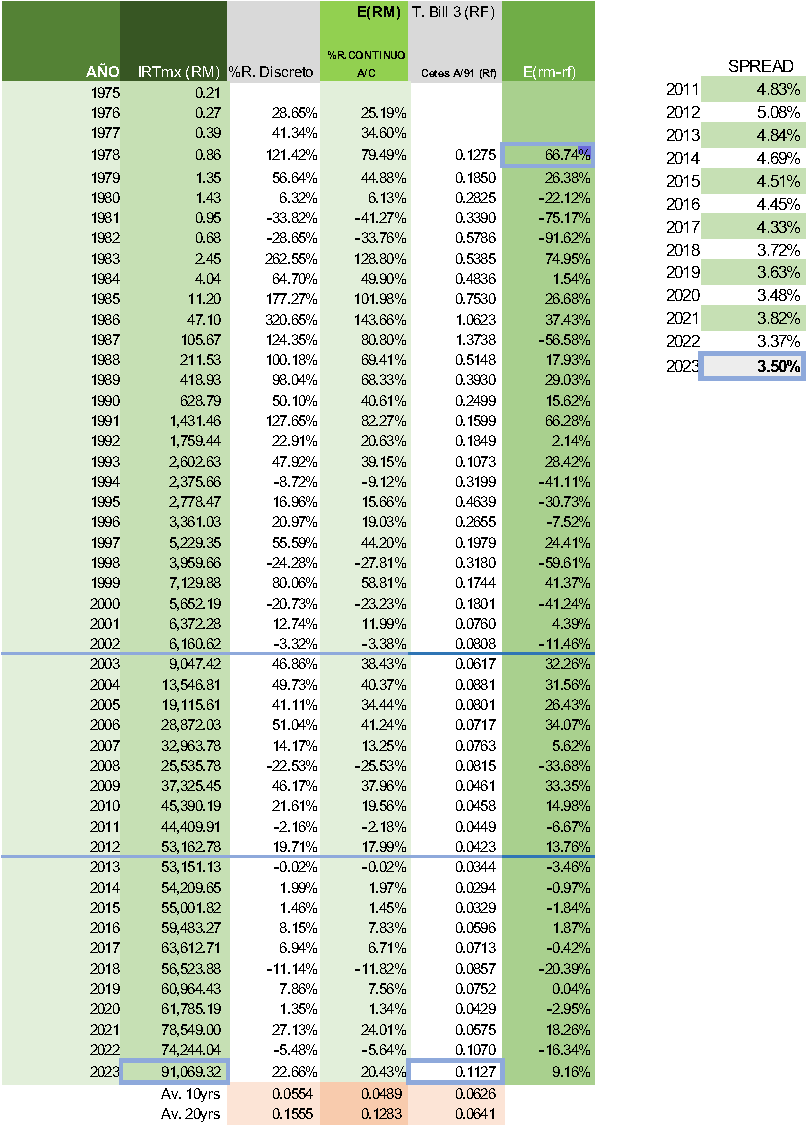
\includegraphics[width=5cm]{imagenes/erp}
\end{figure}

\textcolor{principal}{Riesgo Pa\'is (CRP).} Corresponde al riesgo pa\'is de M\'exico, seg\'un indicador de JP Morgan. Se considera un pron\'ostico para la prima de riesgo adicional de 361 puntos base.

\begin{figure}[H]
\centering
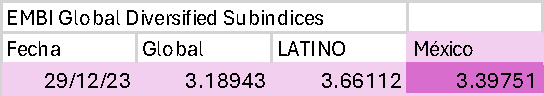
\includegraphics[width=8cm]{imagenes/crp}
\end{figure}

Estimaci\'on del costo de capital (Ke), con un resultado de \textcolor{principal}{16.08\%.}

\begin{figure}[H]
\centering
\includegraphics[width=10cm]{imagenes/ke}
\end{figure}

\textcolor{principal}{Costo de la deuda (Kd).} Para determinar la tasa WACC, se consider\'o el costo impl\'icito de la deuda de la organizaci\'on, seg\'un las cifras de sus libros contables:

\begin{figure}[H]
\centering
\includegraphics[width=10cm]{imagenes/kd}
\end{figure}

\newpage

\textcolor{principal}{Estimaci\'on de la WACC}. Como resultado de las consideraciones anteriores, se estima una WACC en t\'erminos nominales y despu\'es de impuestos de 13.43\%.

\begin{figure}[H]
\centering
\includegraphics[width=10cm]{imagenes/wacc}
\end{figure}

\subsection{M\'ETODO DE CAPITALIZACI\'ON MEDIANTE PERPETUIDAD CRECIENTE.}

\textcolor{principal}{An\'alisis Hist\'orico de los Ingresos.} Se llev\'o a cabo el an\'alisis hist\'orico de los ingresos del negocio por el periodo de 2016 a 2020, con el objeto de poder determinar un pron\'ostico de corto plazo en los ingresos proyectados del negocio; seg\'un se aprecia:

\begin{figure}[H]
\centering
\includegraphics[width=17cm]{imagenes/Picture1}\\
\includegraphics[width=10cm]{imagenes/Picture2}
\end{figure}

\textcolor{principal}{Estimaci\'on del Flujo de Operaci\'on Neto del negocio (NOPAT).} El valuador llev\'o a cabo la estimaci\'on del flujo de caja del negocio antes de reinversi\'on, con un resultado de \$2'007,716.00 MXN a 2020; seg\'un se aprecia:

\begin{figure}[H]
\centering
\includegraphics[width=17cm]{imagenes/nopat}
\end{figure}

\subsubsection{PROYECCI\'ON FINANCIERA.}
\textcolor{principal}{Capitalizaci\'on mediante Perpetuidad Creciente.} Se determin\'o un pron\'ostico de ingresos para el a\~no 2021, basado en el an\'alisis estad\'istico del periodo de 2016 a 2020; habi\'endose tomado la media artim\'etica de dicha muestra con un resultado de \$327'650,337.00 MXN. A su vez, se tom\'o como pron\'ostico para el margen operativo del negocio el 5.45\% proveniente del hist\'orico del ER de la sociedad a 2020, obteni\'endose un NOPAT de \$17'852,590\footnote{La empresa no ha utilizado el escudo fiscal al contar a\'un con p\'erdidas acumuladas por amortizar.}.  A continuaci\'on, se infiri\'o la tasa de reinversi\'on del negocio para poder calcular as\'i un Flujo de Caja Libre a la Firma esperado para 2020, cuyos resultados se aprecian en dos escenarios elegidos de capitalizaci\'on:\\


\textcolor{principal}{Escenario 1:} Se utiliz\'o el FCFF como indicador financiero para la capitalizaci\'on, con una tasa de 19.73\%\footnote{Con el objeto de impactar un mayor riesgo al primer escenario de capitalizaci\'on se utiliz\'o la ke como una tasa ``estresada'' (distressed rate), en vista de la  alta incertidumbre en el pron\'ostico del Flujo de caja libre ante la situaci\'on financiera actual negocio.}  anual (Ke) y un crecimiento de 7.29\% anual\footnote{Como resultado de la encuesta de expectativas de los analistas del sector privado de Banxico}:

\begin{figure}[H]
\centering
\includegraphics[width=17cm]{imagenes/escenario1}\\[1cm]


\textcolor{principal}{Valor de la Firma: \$60'025,692.00 MXN.}
\end{figure}

\espacio{1cm}
\textcolor{principal}{Escenario 2:} Se utiliz\'o el NOPAT como indicador financiero para realizar la capitalizaci\'on, con  una tasa de capitalizaci\'on normalizada de 17.13\% anual (Ke\footnote{Se normaliz\'o el componente conocido como Beta, al cual se le aplic\'o un efecto del 13\% en la tasa fiscal del sector al despalancar la tasa, y se le incorpor\'o un efecto de tasa marginal del 30\% de ISR aplicable a M\'exico como escudo fiscal, asumiendo las p\'erdidas como un evento no recurrente en dicho escenario.}) y un crecimiento de 7.29\% anual como el escenario anterior:

\begin{figure}[H]
\centering
\includegraphics[width=17cm]{imagenes/escenario2}\\[1cm]


\textcolor{principal}{Valor de la Firma: \$124'565,484.00 MXN.}

\end{figure}

\subsubsection{M\'ETODO DE VALUACI\'ON RELATIVA.}

\textcolor{principal}{Muestra de Mercado de Comparables de Cotizaci\'on (Trading Multiples o PEERS)}. Se aplic\'o el enfoque de mercado con base en 2 indicadores:\\

\begin{figure}[H]
\centering
\includegraphics[width=17cm]{imagenes/peers1}
\end{figure}

Se tom\'o como pron\'ostico de la muestra anterior, el m\'ultiplo de valor respecto de flujos de operativos del Sector (EV to EBITDA), con una estimaci\'on de 10.11x\footnote{Percentil 25 de la muestra.}  veces los ingresos:

\begin{figure}[H]
\centering
\includegraphics[width=10cm]{imagenes/peers2}
\end{figure}



Se tom\'o como pron\'ostico de la muestra anterior el m\'ultiplo de valor respecto de flujos operativos del Sector (FWD Price to Book Value x), con una estimaci\'on de \textcolor{principal}{2.02x}\footnote{Percentil 25 de la muestra.} veces el valor en libros.\\

\espacio{2cm}

\subsection{Valor del negocio en marcha.} El valuador llev\'o a cabo 2 ejercicios de capitalizaci\'on por m\'ultiplos para la estimaci\'on del valor razonable de la empresa, conforme al enfoque de mercado; seg\'un se aprecia:

\begin{figure}[H]
\centering
\includegraphics[width=10cm]{imagenes/Picture3}
\end{figure}

\subsubsection{VALOR RAZONABLE PONDERADO DEL NEGOCIO EN MARCHA, CON CIFRAS AL 31/12/2020}

A continuaci\'on se concluye el valor razonable de la firma (\textit{Firm Value}), a la fecha de valores, habi\'endose dado la siguiente importancia a los modelos en la ponderaci\'on: 
\begin{enumerate}[i)]

\item Un peso del 20\% al modelo de Capitalizaci\'on directa por Flujos de Caja Libre (FCF), \item  Un peso del 20\% al modelo de Capitalizaci\'on directa por Flujo de Operaci\'on Neto (Nopat), 
\item  Un peso del 40\% al modelo de M\'ultiplos de Cotizaci\'on de Valor de Empresa a Flujo Operativo (PEERS 1), y 
\item Un peso del 20\% al modelo de M\'ultiplos de Cotizaci\'on de Valor de empresa a Libro Contable (PEERS 2); seg\'un se aprecia:
\end{enumerate}

\begin{figure}[H]
\centering
\includegraphics[width=12cm]{imagenes/Picture4}\\

\textcolor{principal}{Valor de la Firma al 31/12/2020:}\textbf{\$121'108,754.00 MXN}
\end{figure}

\espacio{1cm}

\subsubsection{VALOR RAZONABLE DEL CAPITAL ACCIONARIO, CON CIFRAS AL 30/03/2021.}
 A continuaci\'on se concluye el valor razonable del capital accionario (Equity Value), a la fecha de valores:

\begin{figure}[H]
\centering
\includegraphics[width=12cm]{imagenes/Picture5}\\

\textcolor{principal}{Valor del Capital Accionario al 31/12/2020:}\textbf{\$62'648,006.00 MXN.}
\end{figure}

\subsection{VALUACI\'ON FINANCIERA DE ACTIVOS INTANGIBLES}

\subsubsection{ENFOQUE RESIDUAL PARA LA ESTIMACI\'ON DEL VALOR DE LA MARCA}

\textcolor{principal}{Aplicaci\'on del m\'etodo residual.} El perito valuador aplic\'o la metodolog\'ia residual para determinar el valor razonable del capital marcario de la empresa, habiendo restado al valor razonable de la firma el valor del activo total ajustado a 2020 (\$20'756,472.00 MXN) seg\'un se muestra:

\begin{figure}[H]
\centering
\includegraphics[width=8cm]{imagenes/Picture6}\\[1cm]

\textcolor{principal}{VALOR DEL CAPITAL MARCARIO}\\


\textcolor{principal}{``D DEGLOEMA Desarrolladora''\textregistered al 31/12/2020:}\\[1cm]

\begin{minipage}{8cm}
\begin{center}
\textcolor{principal}{\$100'352,282.00 MXN. }\\

\textcolor{principal}{Cien millones, trescientos cincuenta y dos mil,}\\
\textcolor{principal}{ trescientos cincuenta y dos pesos 00/100 M.N.}
\end{center}
\end{minipage}
\end{figure}
\espacio{1cm}

